\section{Uncertainties}\label{sec:hmmSyst}

\subsection{Uncertainty of background model}\label{sec:hmmBkgUncert}

The background model $f_\text{B}(\muu)$ described in Section \ref{sec:hmmBkg} provides an estimate of background multiplicity in $\muu\in[120,130]$~GeV based on a fit to data.
This estimate is subject to particular statistical sampling that has produced observed data, impacting the resulting fitted function.
The degree to which such fluctuations result in changes to the estimated background defines an uncertainty $\sigma_\text{b}$ on that estimate.

The procedure to estimate $\sigma_\text{b}$ is based on fits to an ensemble of pseudo-datasets.
First, the data distribution is fit following the procedure in Section \ref{sec:hmmBkg} in order to produce a nominal PDF shape.
Then, the nominal PDF is randomly sampled to produce a pseudo-dataset of observations with the same multiplicity as the observed data.
Each pseudo-dataset is fit by the $f_\text{B}(\muu)$, and the background expectation is computed.
The standard deviation of background expectations from all the pseudo-datasets is a measure of $\sigma_\text{b}$.

\begin{table}[htp]
\caption{Uncertainties on the number of background events with invariant-mass in $\muu\in[120,130]$~GeV.}
\begin{center}
\begin{tabular}{l r}
\toprule
Category & $\sigma_\text{b}$ [\%] \\
\midrule
    3-Lepton               & 5.61 \\
    4-Lepton               & 7.80 \\
\midrule
    4-Lepton High-Purity   & 10.06 \\
    3-Lepton High-Purity   & 8.95 \\
    3-Lepton Middle-Purity & 6.06 \\
\bottomrule
\end{tabular}
\label{tab:hmmSigmsB}
\end{center}
\end{table}

The uncertainty $\sigma_\text{b}$ is measured for each of the inclusive and exclusive categories under analysis.
The size of the ensemble of pseudo-toys used is one thousand for each measurement.
The resulting values are listed in Table \ref{tab:hmmSigmsB}.


\subsection{Reweighted Background Shape}\label{sec:hmmRw}

The division of the inclusive categories into sub-categories based on the MVA discriminant reduces the number of expected background events in those categories.
Simultaneously, this reduces the number of simulated background events that appear in those categories.
When this happens, statistical fluctuations in the simulated background become more significant compared to the overall size of the dataset, resulting in bumpy \muu distributions.
This undermines this approximation that the simulated background models the underlying PDF that generates background events.
To counteract this, a reweighting procedure is used to map the background simulation shape from the inclusive categories onto the exclusive categories defined after the MVA cuts.

The reweighting procedure is concerned with the differential \muu shape of the background in the inclusive categories, $B_\text{incl}(\muu)$, and the exclusive categories, $B_\text{excl}(\muu)$.
The ratio is defined between these in each of the exclusive categories, $R=\frac{B_\text{incl}(\muu)}{B_\text{excl}(\muu)}$.
A second degree polynomial is used to define the PDF in Equation \ref{eqn:hmmRw}.
\begin{equation}\begin{split} \label{eqn:hmmRw}
f_R(x)=&1+x*c_0+c 1*(x)^2 \\
x=&\frac{\muu-110}{50} \\
\end{split}\end{equation} 
Here, \muu is measured in GeV.
This polynomial has two free parameters $c_0$ and $c_1$, as well as the overall normalization.
The Equation \ref{eqn:hmmRw} is fit to the ratio $R$ for each of the exclusive categories.

\begin{figure}[h!]
\captionsetup[subfigure]{position=b}
\centering
\subfloat[][]{{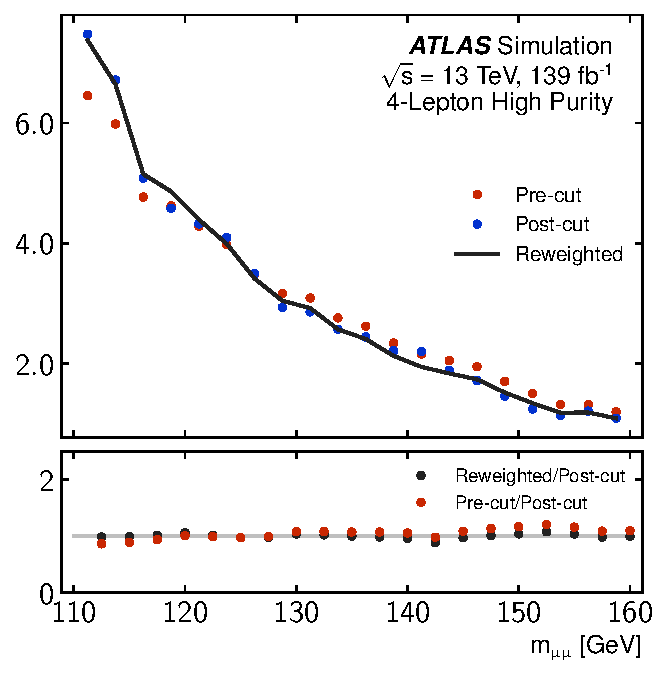
\includegraphics[width=0.32\textwidth]{figures/hmm/reweight/4lep0.pdf}}}
\subfloat[][]{{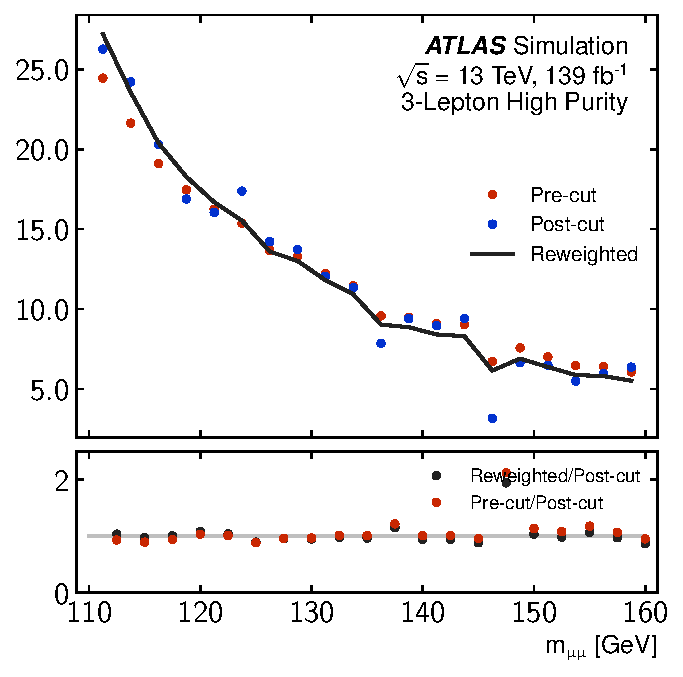
\includegraphics[width=0.32\textwidth]{figures/hmm/reweight/3lep0.pdf}}}
\subfloat[][]{{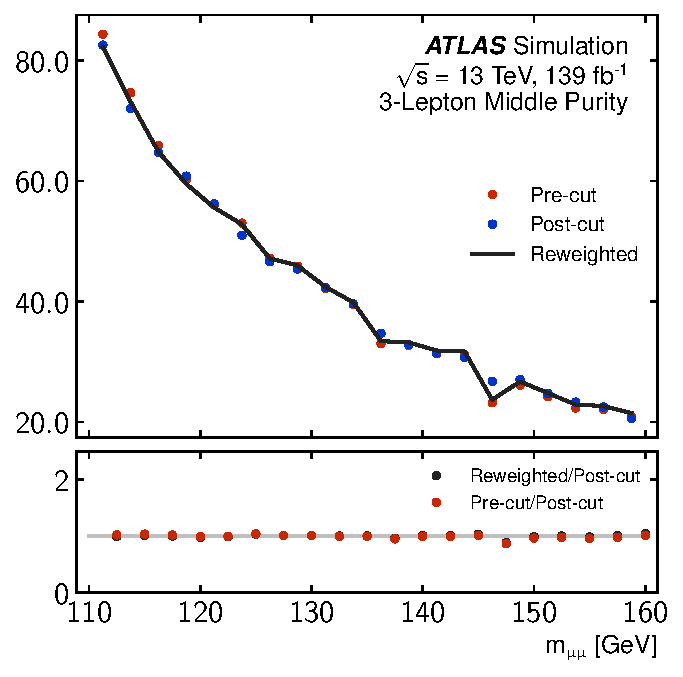
\includegraphics[width=0.32\textwidth]{figures/hmm/reweight/3lep1.pdf}}}
\caption{Illustration of the steps of the reweighting procedure shown for the exclusive categories: 4-lepton high-purity (a), 3-lepton high-purity (b), and 3-lepton high-purity (c).}
\label{fig:hmmRw}
\end{figure}

Figure \ref{fig:hmmRw} shows the reweighting procedure applied to the simulated diboson background in each category.
First the polynomial of Equation \ref{eqn:hmmRw} is fit to the ratio $R$ in each category.
These ratios are shown in the lower half of the figures in red.
The inverse of the polynomial is then convolved with the exclusive distribution, shown in red, to produce a shape similar to the exclusive distribution, shown in blue.
The reweighted shape, shown in black dots, conforms to the shape of the exclusive distribution.
The reweighted shape is also smoother than the exclusive simulation shape due to the larger number of events present in its dataset.
This feature will be helpful in the subsequent measurements of uncertainties.

\subsection{Spurious Signal Uncertainty}

When the S+B model of Equation \ref{eqn:hmmSbFunc} is fit to a dataset, the fitted value of \mus is the signal strength for which the dataset is most likely.
This is interpreted as a measure of the signal strength found in that dataset. 
\footnote{The distinction is subtle, but essential in frequentest statistics.}
When fit to the underlying background PDF, it is ideal for signal strength to be measured at \mus=0.
A deviation from this corresponds to the spurious measurement of signal in a dataset in which it does not exist.
This bias is named \emph{spurious signal}, or \nss, and is the dominant uncertainty associated with this analysis.

It is not a straightforward task to measure the spurious signal associated with a model because the underlying background distributions are unknown. 
An approximation of \nss may be made from the \mus measured when fitting the S+B model to the simulated background dataset.
This makes the implicit assumption that the discretely simulated dataset accurately represents the true underlying background PDF.
Statistical fluctuations in the simulated background limit the accuracy of this assumption.
Instead, fits of the model to the simulated background shape are interpreted as upper limits on the size of \nss, since the recovered \mus includes both the true \nss as well as a measurement of the statistical power of the simulation.
Therefore instead of measuring \nss, a procedure is designed to constrain the size of the spurious signal. 

\begin{figure}[h!]
\captionsetup[subfigure]{position=b}
\centering
\subfloat[][]{{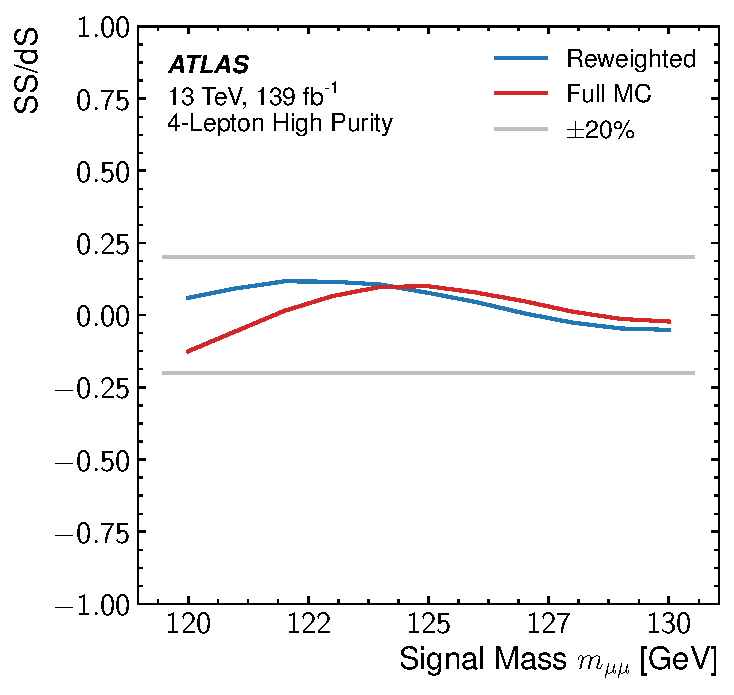
\includegraphics[width=0.32\textwidth]{figures/hmm/ss/ss-4lep0.pdf}}}
\subfloat[][]{{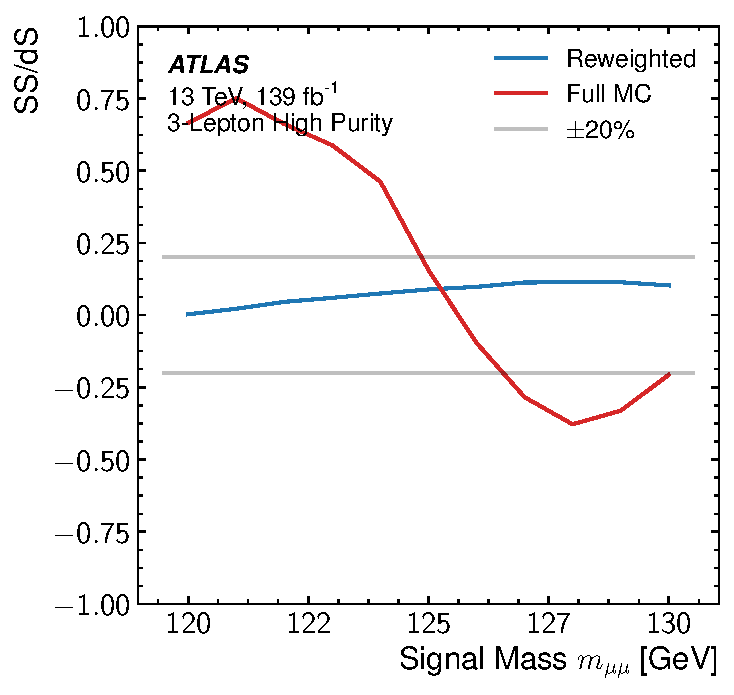
\includegraphics[width=0.32\textwidth]{figures/hmm/ss/ss-3lep0.pdf}}}
\subfloat[][]{{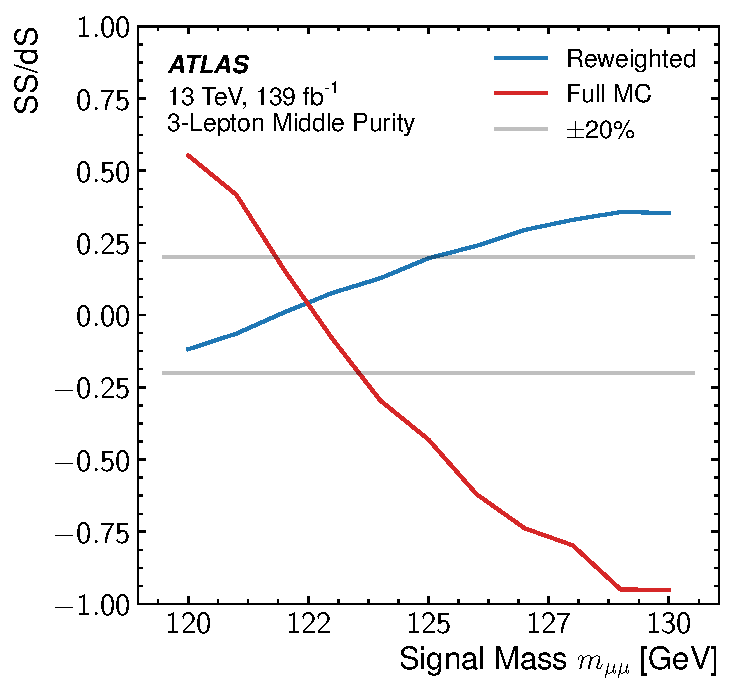
\includegraphics[width=0.32\textwidth]{figures/hmm/ss/ss-3lep1.pdf}}}
\caption{Measurements of the spurious signal relative to the statistical uncertainty on that measurement, $\nss/dS$, shown as a function of signal mass \muu. The measurements are shown in three exclusive categories: 4-lepton high-purity (a), 3-lepton high-purity (b), and 3-lepton high-purity (c). The measurements are made both on the smoothed reweighted background distributions (blue), and the fully simulated background distributions (red). The improvement when using the reweighted distribution is evident in the smaller measured spurious signals.}
\label{fig:hmmSsScan}
\end{figure}

% Scanning signal mass
The result of fitting the S+B model to the background simulation depends strongly on the number of events simulated with invariant mass \muu=125~GeV. 
This is because the signal component of that model peaks sharply in that region.
Since this number of events is subject to statistical fluctuations, the measured \nss is subject to these.
The statistical fluctuations may act to counterbalance the true \nss, resulting in an underestimate of the spurious signal.
A series of alternative S+B models are defined with identical signal components offset by some invariant mass to avoid this.
These are produced with peaks in the range $\muu\in[120,130]$~GeV.
Each S+B model is fit to the same background distribution, which exposes the signal component to different statistical fluctuations.
The relative spurious signal $\nss/dS$ is defined as the measured \mus as a fraction of the statistical constraint on \mus.
This is plotted as a function of signal mass \muu in Figure \ref{fig:hmmSsScan}.
A smooth evolution of the relative spurious signal is an indication that the \nss is measured consistently.

% Smoothed templates
The plots in Figure \ref{fig:hmmSsScan} show the relative spurious signal measured from the simulated background exclusive categories, using both the fully simulated datasets and the reweighted datasets described in Section \ref{sec:hmmRw}.
Here the benefit of using the smoother background representation is seen since, in general, the $\nss/dS$ measured on the reweighted distribution has a smaller magnitude than the fully simulated distribution.
The result with the fully simulated dataset is included for illustration but is not used further.
The maximum absolute value of \nss measured in the range $\muu\in[120,130]$~GeV is taken to define the limit on the spurious signals.
This measurement is performed both in the inclusive and exclusive categories.
These are given in Table \ref{tab:hmmSs}.
Together these define the leading uncertainties on the measured signal strength, \mus. 

\begin{table}[htp]
\caption{Estimates of the spurious signal in each category. First max$(|\nss/ds|)$ is the absolute value of the spurious signal divided by the statistical uncertainty on the measurement, maximized amongst signals with invariant masses in the range $\muu\in[120,130]$~GeV. Next max(\nss) provides the same number without the denominator.}
\begin{center}
\begin{tabular}{l r r r}
\toprule
Category & max$(|\nss/ds|)$ & max(\nss) \\
\midrule
3-Lepton & 0.391 & 1.674 \\
4-Lepton & 0.114 & 1.354 \\
\midrule
3-Lepton High-Purity & 0.114 & 0.458 \\
3-Lepton Middle-Purity & 0.357 & 2.145 \\
4-Lepton High-Purity & 0.117 & 1.108 \\
\bottomrule
\end{tabular}
\label{tab:hmmSs}
\end{center}
\end{table}

\subsection{Experimental and Theoretical Uncertainties}

Uncertainty on the signal simulation arises from limited knowledge of theoretical and experimental that determine it. 
The primary consequence of this uncertainty is that the number of events expected to be reconstructed from the Standard Model VH signal processes is not precisely known.
Theoretical uncertainties cause it to be uncertain how many events the Standard Model may predict.
Experimental uncertainties lead to uncertainty in how many events may be reconstructed, given the standard model's prediction.
In each case, the impact on the amplitude of the signal shape in each category is estimated with a comparison to a signal simulated under a variation corresponding to the theoretical and experimental uncertainties.

The primary sources of theoretical uncertainty on signal production are well studied \cite{higgsCross}.
The largest is on the scale of the strong coupling $\alpha_s$, which leads to changes in the signal amplitude ranging from 3.1-3.5\%.
Next is uncertainty due to the choice of the parton distribution function, with amplitude effects that range from 2.1-2.8\%.
The uncertainty on the branching ratio of the Higgs decaying to two muons is 1.23\% \cite{higgsCross}.
These are all significantly smaller than the spurious signal uncertainty.
This analysis is formulated to make distinctions between signal+background and background-only hypotheses.
In this formulation, there is no uncertainty on the signal model itself, but instead, these uncertainties describe a range of alternative signal models that may be tested independently.

Experimental uncertainty on signal production dictates the uncertainty in efficiency to reconstruct signal events. 
Although this is primarily due to systematic uncertainties related to muon detection, systematics related to election, jet, and \met are also considered.

The primary uncertainties are related to muon reconstruction.
Muon momentum scale and resolutions are measured by three systematics: MUON\_SCALE, MUON\_MS, and MUON\_ID. 
The latter two are uncertainties on the resolutions from the MS and ID measurements.
There is also uncertainty on the efficiency of isolation, reconstruction, trigger, and the track-to-trigger-association (TTVA) \cite{muonReco}.
These efficiencies are measurements in their own right, and the corresponding uncertainties are broken down into systematic (SYS) and statistical (STAT) uncertainties.
% https://cds.cern.ch/record/2665704/files/ATL-COM-PHYS-2019-176.pdf
% Electron
Measurements of energy and resolution are modeled in simulated signal samples based on careful studies \cite{elecReco}.
The uncertainties on both energy and resolution lead to small uncertainties on the signal amplitude.
% PRW
The simulated dataset is scaled by a factor that reflects the efficiency loss due to pileup effects in data.
This introduces a systematic uncertainty called Pile Up Reweighting.
% MET
Uncertainties on the scale and resolution of \met are measured as well.
% Jets
The uncertainties related to jets impact signal yields primarily through the b-jet veto.
These depend on b-tagging efficiency, the uncertainty in the number of tracks associated with the jets, and the jet reconstruction efficiency, energy scale, and resolution.
These are summed in quadrature and counted as a combined ``jet'' systematic.

\begin{table}[htp]
\caption{Experimental systematic uncertainties on the fractional change induced by a systematic on the signal yield in a specific category.}
\begin{center}
{\small
\begin{tabular}{l r r r}
\toprule
Systematic Uncertainty   & \centered{4-Lepton\\ High-Purity [\%]}   & \centered{3-Lepton\\ High-Purity [\%]}  & \centered{3-Lepton\\ Middle-Purity [\%]}   \\
\midrule
 Muon ISO Efficiency STAT   & 0.04   & 0.04   & 0.03   \\
 Muon ISO Efficiency SYS   & 0.41   & 0.42   & 0.42   \\
 Muon RECO Efficiency STAT   & 0.18   & 0.18   & 0.18   \\
 Muon RECO Efficiency SYS   & 0.78   & 0.78   & 0.72   \\
 Muon Trigger Efficiency STAT   & 0.09    & 0.12   & 0.12   \\
 Muon Trigger Efficiency SYS   & 0.16    & 0.21   & 0.23   \\
 Muon TTVA Efficiency STAT   & 0.04   & 0.04   & 0.04   \\
 Muon TTVA Efficiency SYS   & 0.01   & 0.01   & 0.01   \\
 Muon ID   & -0.00    & -0.04    & -0.04   \\
 Muon MS   & -0.04    & -0.00    & -0.01   \\
 Muon SCALE   & -0.08    & -0.11    & -0.07   \\
 \midrule
 Electron Resolution   & 0.04   & -0.07   & 0.09   \\
 Electron Scale   & 0.06   & -0.07   & 0.13   \\
 \midrule
 Jet & 0.64 & 5.06 & 1.80 \\
 \met & 0.03 & 0.30 & 0.11 \\
 Pile Up Reweighting   & -0.64   & -1.16   & 0.34   \\
 \midrule
 Total & 1.30  & 5.28 & 2.05 \\
\bottomrule
\end{tabular}
\label{tab:hmmExpUncert}
}
\end{center}
\end{table}

These are summarized in Table \ref{tab:hmmExpUncert}.
Each number describes the impact on the signal amplitude due to a $1\sigma$ shift in the corresponding experimental quantity in the simulation.
The combined experimental uncertainties are substantially smaller than the spurious signal uncertainty.

Finally, the uncertainty on the integrated luminosity of the dataset is 2.7\% \cite{LUCID2}.



